\section{Introduction}

A drug that reaches the bloodstream does not stay the compound that was administered. Enzymes,
chiefly in the liver, convert it into other compounds carrying their own activity, toxicity and
persistence: a metabolite can be the agent that makes a drug work, as with the antiviral prodrugs
activated by phosphorylation, or the agent that makes one fail, as with the reactive intermediates
behind several withdrawals. The same question arises outside the clinic, where what an
environmental chemical becomes in an organism determines how far it travels and how long it lasts.
Knowing which metabolites will form, as chemical structures rather than as a count or a rate, is
therefore useful early, when a compound exists only on paper.

Two families of method now dominate. Rule-based systems, among them SyGMa \citep{Ridder_2008},
BioTransformer \citep{Djoumbou_Feunang_2019}, GLORY and GLORYx \citep{de_Bruyn_Kops_2019,
de_Bruyn_Kops_2020} and MetaTox \citep{Rudik_2017}, encode known biotransformations as reaction
templates and enumerate the products of applying them. Sequence-to-sequence systems, among them
MetaTrans \citep{Litsa_2020} and MetaPredictor \citep{Zhu_2024}, treat the problem as translation.
Recent work extends both lines: a chemical language model \citep{Larsson_2025}, a mechanistically
informed graph framework \citep{Zhou_2025}, a server predicting pathway, site and product together
\citep{Zhou_2026}, and a preprint predicting all three jointly \citep{Chavan_2026}. The two
families are used for different reasons. A template names the transformation it applied and the
atoms it acted on, so a chemist can see why a structure was proposed and reject it on mechanistic
grounds; that is what makes rule-based systems usable in a discovery workflow, where a prediction
has to be defended to a medicinal chemist rather than only scored. A sequence model is not built to
say that, and is expected instead to reach chemistry no template bank encodes.

What is missing is not another predictor but a way to tell these apart. The usual measure is
recall: the fraction of the metabolites recorded for a compound that a system returns. That
fraction depends on two decisions made outside the model. The first is what counts as a match,
since two chemical structures can denote the same molecule while differing in how a hydrogen is
placed or how a ring is drawn. The second is how many candidates the system is allowed to return,
since any system recovers more of the answer if permitted to list more guesses. Published
predictors differ on both and report them inconsistently, and the difference is not small: the ones
compared here emit between \numEmittedBiotransformer{} and \numEmittedSygma{} candidates
per substrate by default, so a recall figure quoted for one is not on the scale of a recall
figure quoted for another. Independent evaluations of these tools report the same obstacle
\citep{Boyce_2022, Scholz_2023, Gao_2026}.

That a comparison can turn on an undeclared choice is not new, and two recent statements of it
bound what this paper adds. \citet{Ash_2025} give a protocol for method comparison in small-molecule
drug discovery, arguing that a difference should be shown practically significant rather than
merely significant, and prescribing how a comparison ought to be set up. \citet{Ozcelik_2025} show
what happens when it is not, in generative design: the size of the library and the choice of metric
reorder the models. The gap between the two is where this work sits. A protocol tells an author
what to declare; a demonstration on generative metrics does not transfer to recall against an
incomplete annotation, where the axis that reorders methods is how many candidates each may emit
and no analogue of it exists in distributional metrics. What is offered here is the measurement in
that setting: the axes swept, the whole grid printed, and a bound on what any bank mined from this
corpus could reach.

This work addresses that. We present GRAIL (Graph-scored Rule Application with Inspectable
Localisation), a metabolite structure predictor built from a bank of reaction templates, a learned
model that selects which templates to apply, and a learned model that ranks the resulting
candidates. Every prediction it emits carries the template that produced it and the atoms that
template acted on, so a chemist can accept or reject a candidate on mechanistic grounds rather
than on a score. We evaluate it with the two decisions above promoted to declared axes: each is
stated and varied across its full range instead of being fixed silently. The comparison is against
\numComparatorsColumnsWord{} published predictors we obtained and ran on the same substrates. It
does not produce a winner: which system leads depends on how many candidates it is allowed to
return, and we report that dependence rather than a single figure. We further measure how much of
the recorded chemistry lies outside the reach of any single template application, and find that
most of what is missing is chemistry the training corpus does not contain, which no template mined
from that corpus could supply.

The article is organised as follows. Section~\ref{sec:methods} describes the corpus, the three
stages of the system and the evaluation protocol. Section~\ref{sec:results} reports the
comparison against published predictors, the contribution of each stage, the sensitivity of the
result to the evaluation choices, a worked example, and the coverage bound.
Section~\ref{sec:discussion} discusses where the advantage lies and what the measurements do not
establish, Section~\ref{sec:limitations} the limitations and
Section~\ref{sec:conclusions} the conclusions. Procedures, ablations and supporting measurements are in the Supporting Information.

\section{Materials and methods}
\label{sec:methods}

\subsection{Which population carries which number}
\label{sec:populations}

The corpus divides into three substrate-disjoint splits: \numSplitTrainSubstrates{} training
substrates carrying \numSplitTrainPairs{} annotated pairs, \numSplitValSubstrates{} validation
substrates carrying \numSplitValPairs{}, and \numSplitTestSubstrates{} test substrates carrying
\numSplitTestPairs{}. The splits are disjoint by substrate, as a held-out figure requires \citep{Joeres_2025, Kretschmer_2025}, and an audit confirms it (Section~\ref{SI-sec:si-corpus}). The pairs are
assembled from ChEMBL \citep{Zdrazil_2024}, DrugBank \citep{Wishart_2018}, MetXBioDB
\citep{Djoumbou_Feunang_2019} and the GLORYx reference set \citep{de_Bruyn_Kops_2020}, at versions
\CorpusVersions{}.

Three populations carry the figures here, and no figure is given without naming one. The
\emph{evaluated test set} is the \numPopulationTestsubs{} test substrates carrying at least one
reference, holding all \numPopulationTestrefs{} references of that split. Both corpus-level
measurements are made on it: the \emph{coverage ceiling}, which is the share of the annotated
references any application of the rule bank could reach at all, and the census of the chemistry the
remainder needs. The \emph{validation draw} is a declared sample of \numValdrawCap{} substrates on which the registered ranking and timing thresholds are checked, because a threshold checked on the population that chose the setting it tests is not a check; Table~\ref{tab:hyp} records the population each prediction was in the event checked on, and Section~\ref{SI-sec:si-register} states that all but one of the ten fixed a threshold in advance and not a population. The
\emph{comparison set} is the \numPopulationN{} substrates every method has an entry for, carrying
\numPopulationReferences{} references, and every comparison against a published predictor is
measured on it.

That third population has a defect worth stating before any number is read on it. It is not a
random quarter of the test split: it is the submission list sent to the comparator that is a web
service, and how those \numPopulationN{} were drawn is recorded nowhere in this repository, which
is the same defect the corpus assembly carries. So the comparison is read again on the whole
evaluated test set, \numPopdefWholesubstrates{} substrates, against the
\numPopdefWholearmsWord{} comparators that ran over all of it
(Section~\ref{SI-sec:si-population}). The wide-budget leads survive that move and the narrower lead
over SyGMa at a budget of fifteen does not, so that one is restricted to the comparison set wherever
it is stated. The move also costs more than it takes. An \emph{arm} here is one column of the comparison, and
this system contributes two of them: the \emph{exhaustive} arm, which applies the whole bank, and
the \emph{interactive} arm, which applies a fixed number of the highest-scoring rules
(Section~\ref{sec:modes}). At a budget of ten the exhaustive arm trails SyGMa by
$\numPopdefExhwholesygmaOneZero$ and MetaPredictor by
$\numPopdefExhwholemetapredictorOneZero$ over the whole set, both intervals excluding zero, where on
the comparison set neither cell separates at all. Neither is therefore among the
\numHolmSeparating{} cells the family-wise correction is applied to, and the
\numHolmLeadsremovedWord{} it removes are leads of this work's.

One property of the assembly bears on everything downstream: the selection that drew records from
the four sources is not recoverable.  The apparatus built on top therefore makes every
step from the corpus onwards reproducible and cannot make that one so. What can be checked instead is a rebuild, which the repository reports substrate by substrate, and the one source held here in full says the selection was not blind to chemistry: the transformation types it kept and those it dropped are differently distributed, and the GLORYx set points the same way without settling it (Section~\ref{SI-sec:si-typeoverlap}).
ChEMBL and DrugBank are the other two sources, neither is held here, and nothing tests them. Every
statement in this paper about what the corpus does and does not contain is a statement about a
corpus assembled that way.

How the corpus was assembled has a consequence for the comparison which no split can remove. Rule-based comparators have
no training set to hold out, and their expert rules may encode the same metabolism reported in
these sources; BioTransformer is built on MetXBioDB, and GLORYx was developed against the
reference set of the same name. Their knowledge therefore overlaps the test substrates by construction, in a direction that
favours them. Both are columns of the comparison, both overlaps are measured in
Section~\ref{SI-sec:si-corpus}, and neither is corrected for: a correction would need a model of
how much of a rule set a reference set produced, which nothing here supplies. The comparison
therefore contains two arms whose development sources this corpus draws on, with the advantage
stated and left in place; the comparison without them is the other three columns.
The remaining three arms are not measured against this corpus and are not thereby cleared:
MetaTox and MetaPredictor publish no development set that could be intersected with it. What is
reported is the one overlap that could be computed, not a survey of all four.

\subsection{Overview}

Each design choice below is given with the measurement that decided it and the prediction it was registered as; those predictions, each with a threshold and a falsification condition fixed before the check, are the \emph{register} (Table~\ref{tab:hyp}).

GRAIL predicts in three stages, each separately inspectable. A generator scores every rule in a
bank of \numBankRules{} reaction templates, written as SMIRKS transformation patterns, against
the substrate. The selected rules are then
applied with RDKit 2022.09.5, and their products are
standardised \citep{Hahnke_2018, Mansouri_2024} and deduplicated. A template that breaks a bond returns more than one species. Every product, and every disconnected
component of it, enters the pool separately provided it has at least \numFragmentFloorWord{} heavy
atoms. That drops a lone leaving group and keeps a small metabolite such as formate. No annotated
metabolite in the evaluated test set is multi-component, so the convention decides what is offered
rather than whether a reference is reached. A scorer scores each
(substrate, candidate) pair, encoding the two molecules as separate graphs rather than as one
merged graph, and the candidates are ordered by a rank fusion of that scorer's and the generator's
orderings.  Every emitted candidate carries the identity of the rule that produced
it and the site at which it fired.

A candidate reachable by several rules, or by one rule firing at several sites, receives a single
score. Writing $R(c)$ for the rules that produce $c$ and $p_r$ for the generator's probability
that rule $r$ applies, the aggregation is noisy-or,
\begin{equation}
p(c) = 1 - \prod_{r \in R(c)} \left( 1 - p_r \right),
\label{eq:noisyor}
\end{equation}
so evidence from independent rules accumulates rather than competing. The independence is an
assumption this bank does not satisfy, since it holds published rule sets verbatim and the mined
half is full of near-duplicates. What that costs is swept over the four aggregation rules
the implementation offers (Section~\ref{SI-sec:si-knobs}).

Both learned stages were trained on a subsample of the training split, fixed when the run was configured and not a consequence of anything measured here, so what the ablations compare (Section~\ref{SI-sec:si-ablations}) is the value of each stage at that training budget rather than at the split's full size. Every setting is in Section~\ref{SI-sec:si-arch}.

\subsection{What this system does not represent}
\label{sec:methods-scope}

Nothing in this pipeline is stereochemistry-aware. The standardiser strips configuration, the
matching criterion is chosen to ignore it, and the annotation carries none, so sulfoxidation,
epoxide hydrolysis and most conjugation are predicted and scored as constitutions. For a predictor
of metabolite structures that is a restriction on what may be asked of it rather than a
technicality: sulfoxide and epoxide configuration carry the pharmacology of several drug classes,
and a system that cannot represent configuration cannot be asked which enantiomer an enzyme makes.
Every recall figure in this paper is therefore recall over constitutions, and the size of what that
sets aside is bounded in Section~\ref{sec:limitations}.

\subsection{Rule bank}

The bank holds \numBankRules{} templates spanning \numBankTypes{} distinct reaction types, where a
type is the multiset of bonds that change between mapped atoms. A template is a mapped SMIRKS,
and \emph{rule} names the same object here and in the released files. The bank is the
deduplicated union of \numAttribNamed{} templates
from three curated collections and \numMinedRules{} mined from the training split alone,
together with \numAttribUnattributed{} that were carried as a fourth curated collection and are
not one: they are an earlier machine extraction from the same annotated pairs, The bank therefore holds two machine extractions and one curated body (Section~\ref{SI-sec:si-bank}). Most of that body is not this work's chemistry: at least \numThirdpartyBorrowed{} of the \numAttribNamed{}, \numThirdpartyBorrowedsharePct{}, appear verbatim in rule sets published by others. What is this work's own is the mining, the ranking and
the measurement, not the writing of the templates, and Section~\ref{SI-sec:si-bank} gives the
counts per rightsholder with the terms each requires. That split is disjoint by substrate and not by molecule, so a training substrate may reappear as a test product; both overlap counts are in Section~\ref{SI-sec:si-corpus}. Each mined template is the reaction centre of one annotated pair, the atoms and bonds that changed, expanded by one bond, and it survives only if applying it to its own source substrate regenerates that pair's product (Section~\ref{SI-sec:si-bank}).

Support is heavily skewed: \numRareSingletonsharePct{} of the mined templates rest on a single
training pair. A rarefaction curve over withheld pairs is still climbing (Section~\ref{SI-sec:si-rarefaction}), so template discovery from this corpus is not finished.

\subsection{Rank fusion}

Both learned stages produce an opinion about each candidate, and their product is scale-sensitive:
if one scorer occupies a narrow range and the other a wide one, the wide one decides the order. The deployed combination is reciprocal rank fusion \citep{cormack2009}, which scores a candidate by the sum over the two scorers of $1/(K + r)$, where $r$ is its rank under that scorer. Only positions enter, so the two opinions
contribute equally whatever their scales. $K = \numFusionkDeployed$ is the value the method was
published with, and it is swept rather than merely disclosed. No constant of \numFusionkFlatfrom{} or more separates from it at output budgets of 5, 15 and 50; at 30 one does, and in the deployed value's favour (Section~\ref{SI-sec:si-knobs}).

The change was registered as prediction P1, with a threshold of $+\numHSevenThreshold$ fixed
before it was checked. Evaluated on a validation draw where the fusion had not been selected, it
gives $+\numHSevenDiff$ $[+\numHSevenLo, +\numHSevenHi]$. On the capped pool the deployed system
ranks, the same contrast is $+\numHSevenDeployed$, because the cap and the fusion recover
overlapping ground (Table~\ref{SI-tab:si-ranking}).

\subsection{Pool cap}

Before fusion the pool is truncated by generator score, a quantity available before any pair graph
is built:
\begin{equation}
\hat{C}(s) = \operatorname*{arg\,top}_{c \in C(s)}{}^{\,\numHNineCap} \; p(c),
\end{equation}
where $C(s)$ is everything the applied rules enumerate.  The
fusion ranks over whatever survives, so removing a candidate changes the rank every other receives,
and truncation can therefore raise recall rather than only bound it. The cap raises recall by $+\numHNineDiff$ $[+\numHNineLo, +\numHNineHi]$ and takes the mean pool from \numHNinePoolBefore{} candidates to \numHNinePoolAfter{} (P2, Table~\ref{tab:hyp}). The value was fixed by a stated principle rather than by a search. The cap must be at
least twice the widest output budget reported, so that the widest column is never simply the whole pool,
and 100 is the smallest round number that satisfies it.

\subsection{Rule budget and two operating modes}
\label{sec:modes}

How many templates the generator selects before any is applied is the \emph{rule budget}. It is
not the output budget of Section~\ref{sec:evaluation}, which is how many candidates a system may
return; where this paper writes \emph{budget} unqualified it means that one. The rule budget is one
continuous setting, and the two modes reported throughout are two points on it rather than two
designs. The \emph{interactive} mode applies the \numHOneZeroTopk{} templates the trained
checkpoint records and returns in about a second, which is what a user waiting at a web form
requires; the \emph{exhaustive} mode applies the whole bank, the \numBankParses{} of
\numBankRules{} templates that parse, and takes tens of seconds. The interactive value is where
the released checkpoint was trained, which is a fact about how the run was configured and not an
argument for the number, so the curve either side of it is measured on validation
(Section~\ref{SI-sec:si-budget}). What the difference buys was fixed in advance as prediction P3 and, on validation, came in under its ceiling (Table~\ref{tab:hyp}).

\begin{table}[t]
\centering\footnotesize
\begin{tabular}{lrr}
\toprule
 & interactive & exhaustive \\
\midrule
rules applied & 30 & 7{,}580 \\
candidates, mean & 16.5 & 98.0 \\
candidates, median & 14.0 & 100 \\
seconds, median & 0.39 & 5.28 \\
seconds, mean & 2.36 & 52.77$^{\dagger}$ \\
seconds, 90th pct & 2.59 & 89.78$^{\dagger}$ \\
seconds, slowest & 231.01 & $>600$$^{\dagger}$ \\
\bottomrule
\end{tabular}
\caption{The two operating modes: rules applied, candidates returned and wall-clock time. Every
row but the two marked $^{\dagger}$ is measured on the validation draw, 294 substrates for
the interactive mode and 293 for the exhaustive one, which lacks a pool for one
of them; the median seconds are over those populations. Candidates are
what a caller receives: deduplicated by matching key and capped at
100. Times cover everything before the filter. $^{\dagger}$ marks a statistic that is both censored and measured on a different population: a sampled timing sweep of 106 substrates, on which the exhaustive mode exceeds a 600-second deadline for 11, 10.4\%, so its mean and ninetieth percentile are taken over the 95 that finished. Those two are lower bounds against that sweep, where censoring removes the slowest; against the whole draw the sweep's design pushes the other way, since it over-represents large substrates on purpose, and the net of the two is not established here. That sweep is drawn as every 3rd substrate of that draw by heavy-atom count plus the largest 12 outright, so it over-represents the sizes where the deadline bites: 9 of the 11 non-completions are among those 12, and the rate the whole draw would show is about 15 in 294, 5.1\%. Its slowest substrate is one of the censored ones, which is why that cell carries the mark as well: a deadline is defined only for the sweep, so a $>$ entry can come from nowhere else, and the two arms' slowest cells are therefore not on the same substrates. On the test split, where no deadline is imposed, it fails on none. Every time here is measured on an unloaded machine and one substrate at a time; the exhaustive median carried to the load of a second arm is larger, and Section~\ref{SI-sec:si-runtime} gives it, derives it from this median rather than measuring it again, and says between which arms the load ratio was taken. The interactive mode's own slowest substrate, 231.01~s, is far above its median, so a service answering a form should impose a deadline and fall back rather than assume the median.}
\label{tab:modes}
\end{table}


On the comparison set the same quantity is $+\numHOneZeroComparison$, past the ceiling. The
discrepancy is reported rather than resolved and it has a reading: at $k \le 10$ the whole bank
buys nothing on either population, and from $k=15$ it buys more the wider the budget, because the
interactive arm runs out of candidates. P3's ceiling is therefore a property of the output budget
requested rather than of the system, and so is the deployed rule budget. Read at an output budget of fifteen the curve is flat past the deployed rule budget; read at an output budget of thirty it is not (Section~\ref{SI-sec:si-budget}).  What that costs to run, and which budget it is worth paying at, is the
Discussion's question rather than this section's.

\subsection{Emission}

A threshold on a score product does not transfer to a rank fusion, which is a rank statistic without scale: at the value this system registered it admits \numEmitByfusion{} candidates of a pool of \numEmitPool{}. The deployed emission is therefore $\hat{C}(s)$ itself, ordered by fusion and truncated by no
threshold, so $|\hat{Y}_s| = |\hat{C}(s)|$. For the interactive mode that length is set by the
rule budget and the substrate's chemistry, and its mean of \numEmittedTrained{} on the comparison
set sits well below any cap. Table~\ref{tab:modes} prints the same quantity on the validation draw, and Table~\ref{SI-tab:si-counts} lists every candidate count in this work with its stage and population. The exhaustive mode differs: its pool is capped at 100 by the cap prediction P2 registers, and
its mean output of \numEmittedBank{} is close enough to that cap that the cap sets its length on
most substrates. That cap is a parameter of this system, it is declared, and it applies to that
arm and not to the comparators. It was registered as prediction P4 and confirmed (Table~\ref{tab:hyp}); its budget ladder was fixed with the prediction and is not the one read elsewhere here.

\subsection{Evaluation}
\label{sec:evaluation}

What decides when a predicted structure counts as one of the references is the
\emph{matching criterion}. It is treated here as a declared axis with five settings: canonical
SMILES equality, the full InChIKey, its stereochemistry-blind first block, Tanimoto similarity of
one over Morgan fingerprints, and a tautomer-aware key that canonicalises tautomers on both
sides. The last is the
default, because the references neither carry stereochemistry nor distinguish tautomers, and
because standard identifiers normalise only a subset of tautomers \citep{Dhaked_2020}. That the
annotation carries no stereochemistry is also a limit on what any of these systems can be asked
for: nothing in this pipeline is stereochemistry-aware, so sulfoxidation, epoxide hydrolysis and
most conjugation are predicted as constitutions and not as configurations. All five are reported for every
comparison, with the levels behind every verdict in Table~\ref{SI-tab:si-criterion-levels}.

A third choice sits behind both declared axes, the matching criterion and the output budget:
how the substrate itself is drawn. Templates are matched against
the structure the corpus stores, and that corpus draws amides as imidic acids, so the choice is not
neutral. It is a deployment question and not only an evaluation one, because a user submits the drawing a chemist would make, and on the substrates the standardiser changes the effect is larger than the pooled figure suggests (Section~\ref{SI-sec:si-dialcond}).
Rebuilding both GRAIL arms with every substrate redrawn moves \numDsweepMoved{} of
\numDsweepCells{} arm-against-comparator verdicts, none of them a lead claimed here.

The arms did not all meet that choice the same way, and the asymmetry belongs here rather than in a
sweep. Of the \numChemArmsWord{} arms, \numChemDrawnstoredWord{} were handed the substrate as the
corpus stores it; MetaTox was not, its submission file re-tautomerising the substrate to the
natural form for \numDialectMetatoxretaut{} of the \numDialectMetatoxn{}. The direction is not neutral, since this bank's mined half requires the imidic reactant more often than the amide, and its size is measured for every arm that can be re-run (Section~\ref{SI-sec:si-presentation}). The whole comparison with every re-runnable arm on the
drawing a user would submit is Table~\ref{SI-tab:si-equalised}, and it moves
\numEqualisedMovedWord{} of the nine verdicts: every arm's level falls or rises with the drawing and
the division between them does not. Table~\ref{tab:sweep} is read in the corpus dialect, in which
every reference is also stored.

The arms are also not held at one enzymatic depth, and no reading here equalises it. SyGMa composes
a phase-one and a phase-two ruleset, BioTransformer is run for one step, MetaTox's depth is neither
ours to turn nor readable, and a mined template may perform more than one enzymatic edit in a single
application, as \numCompositeUnionsharePct{} of this bank's mined templates do
(Section~\ref{SI-sec:si-singlestep}). The depth is swept for SyGMa, whose scenario is a documented
setting, and the lead survives it. BioTransformer's step count is also ours to turn and was not
swept, a decision taken after the matched-length control, which cuts every arm to the comparator's own
list length substrate by substrate, had been read, and stated as such
(Section~\ref{SI-sec:si-comparators}). For those two the difference between the arms is stated
rather than removed, and the wide-budget cells should be read with it in view.

The number of candidates a system is permitted to return is the \emph{output budget}, written
$k$, and it is the second declared axis. Recall at budget $k$ for substrate $s$ with references
$Y_s$ and the first $k$ predictions $\hat{Y}^{(k)}_s$ is $|Y_s \cap \hat{Y}^{(k)}_s| / |Y_s|$. Two aggregations are distinguished
throughout and never mixed within a comparison,
\begin{align}
\mathrm{macro} &= \frac{1}{|S|}\sum_{s \in S}
\frac{|Y_s \cap \hat{Y}^{(k)}_s|}{|Y_s|}, \\
\mathrm{micro} &= \frac{\sum_{s} |Y_s \cap \hat{Y}^{(k)}_s|}{\sum_{s} |Y_s|},
\end{align}
and every figure states which it is. Intervals are a paired bootstrap over substrates: for each of
$B = 10\,000$ resamples $S^{(b)}$ drawn with replacement,
\begin{equation}
\delta^{(b)} = \frac{\sum_{s \in S^{(b)}} \left( h^A_s - h^B_s \right)}
{\sum_{s \in S^{(b)}} |Y_s|},
\label{eq:bootstrap}
\end{equation}
with $h^A_s$ and $h^B_s$ the hits of the two arms. The reported interval is the empirical $2.5$ and
$97.5$ percentiles of $\{\delta^{(b)}\}$. Resampling substrates rather than
predictions is what makes the interval one on the \emph{difference} between two arms read on the
same items. Precision is reported in Table~\ref{SI-tab:si-precision} but is not used to order the systems, because under incomplete annotation a real but unannotated metabolite counts as a false positive against whichever arm predicts it (Section~\ref{SI-sec:si-precision}).

Every method is prevented from returning the substrate itself as one of its own metabolites:
a prediction equal to the substrate is discarded before the budget is applied, for all arms
alike. That is the \emph{parent-drop} convention, and it is swept like the other declared
choices.
It does not favour one over another: the largest effect on recall anywhere in the grid is
\numPdropMaxEffect{} and no cell separates from zero (Table~\ref{SI-tab:si-parentdrop}).

Every interval in this paper is a per-comparison 95\% interval with no family-wise adjustment.
Both readings are reported. Treating as one family the \numHolmTests{} tests the correction was declared over, the two arms against \numSweepFamilycomparatorsWord{} comparators, and applying Holm's correction, \numHolmSurviving{} of the \numHolmSeparating{} cells that separate per comparison still separate; the \numHolmChangedWord{} that do not are marked in Table~\ref{SI-tab:si-intervals}. Of those, \numHolmLeadsremovedWord{} are leads, and every one of the
\numHolmLeadsremovedWord{} is a lead this paper claims somewhere: the exhaustive arm over
MetaTox at $k=30$, over SyGMa and over MetaPredictor at $k=15$, and the interactive arm over
MetaTox at $k=10$. Each is marked where it is claimed. Two
comparators were obtained after that family was fixed, so their contrasts are reported with their
own intervals and are not folded into a correction declared without them
(Section~\ref{SI-sec:si-comparators}).

That leaves the obvious objection, which is that this paper prints more contrasts than the family
covers, and it is answered by measurement rather than by the declaration. Applying the same
correction to every contrast printed anywhere here, \numHolmWidetests{} of them,
\numHolmWidesurviving{} still separate, and it removes \numHolmWideremovesdeclaredWord{} cells the
declared family keeps. Of those \numHolmWideremovesdeclaredWord{},
\numHolmWideleadsremovedWord{} is a lead of this work's, over MetaTox at $k=10$, and the other two
run against it. So the wider
reading costs this paper one cell and gains it two, and neither reading changes the wide-budget
result.

No single budget is privileged. A claim that the system leads is made for a cell only where that
cell's interval excludes zero, and where an ordering is not established the table says so.
Reporting the whole space of defensible analysis choices rather than one chosen
cell is the multiverse and specification-curve discipline \citep{Steegen_2016, Simonsohn_2020},
applied here to the two choices this literature leaves undeclared.

\section{Results}
\label{sec:results}

\subsection{Comparison with published predictors}

\begin{table*}[t]
\centering
\small
\begin{tabular}{rrrrrrr}
\toprule
$k$ & GRAIL exh. & GRAIL int. & MetaTox & SyGMa & MetaPred. & BioTrans. \\
\midrule
1 & 0.0992 & 0.1053 & 0.0406 & 0.1534 & 0.1398 & 0.0722 \\
3 & 0.2301 & 0.2406 & 0.1323 & 0.2887 & 0.2767 & 0.1940 \\
5 & 0.3113 & 0.3203 & 0.2180 & 0.3744 & 0.3549 & 0.2752 \\
8 & 0.4165 & 0.4015 & 0.3113 & 0.4271 & 0.4346 & 0.3414 \\
10 & 0.4556 & 0.4331 & 0.3880 & 0.4556 & 0.4707 & 0.3759 \\
15 & 0.5353 & 0.4797 & 0.5143 & 0.4842 & 0.4797 & 0.4286 \\
20 & 0.5865 & 0.4872 & 0.5519 & 0.4992 & 0.4797 & 0.4421 \\
30 & 0.6526 & 0.4902 & 0.6015 & 0.5068 & 0.4797 & 0.4466 \\
50 & 0.7023 & 0.4902 & 0.6271 & 0.5113 & 0.4797 & 0.4481 \\
\midrule
\emph{mean emitted} & \emph{98.12} & \emph{15.63} & \emph{33.60} & \emph{72.98} & \emph{10.75} & \emph{10.70} \\
\bottomrule
\end{tabular}
\caption{Micro recall at each output budget on the 291 substrates of the comparison set, carrying 665 annotated metabolites. The last row gives the mean number of candidates each method emits, before any budget is applied: it is a property of the method and not of this table, and for two of the comparators it is larger than the widest budget shown. A prediction equal to the substrate is dropped before the budget for every method alike.}
\label{tab:sweep}
\end{table*}


\begin{figure}[t]
\centering
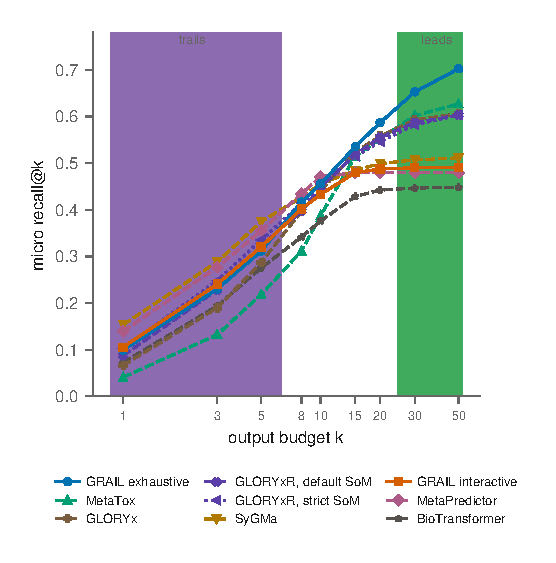
\includegraphics[width=\columnwidth]{fig_sweep}
\caption{Micro recall against output budget on the \numPopulationN{} substrates of the
comparison set. Shading marks the budgets at which the better GRAIL arm trails the strongest
comparator with the paired interval excluding zero (lavender) or leads on the same condition
(green); budgets where neither separates are unshaded. The shading is read at a nominal budget,
which is not a list length: of the comparators the green region leads, most do not survive
matching on realised length (Table~\ref{tab:si-matched}).}
\label{fig:sweep}
\end{figure}

Figure~\ref{fig:sweep} and Table~\ref{tab:sweep} are the comparison on the \numPopulationN{}
substrates of the comparison set. Read against the strongest comparator at each budget it divides
in three rather than resolving into an ordering. Every difference behind that division, with its paired interval, is
Table~\ref{SI-tab:si-intervals}.

GRAIL trails with the interval excluding zero at $k=1$, $3$ and $5$, where SyGMa leads:
\numSweepTrainedOne{} against SyGMa's \numSweepSygmaOne{} at $k=1$. Two of those three, at $3$ and $5$, do
not survive the family-wise correction either.  The two banks
are not independent, and the reading depends on it. \numSygmaInside{} of SyGMa's
\numSygmaRules{} published rules are present in this bank verbatim, so what separates at those
budgets is an ordering over chemistry the two systems largely share. Neither side separates at $k=8$ and
$10$, where MetaPredictor leads, nor at $k=15$ and $20$. GRAIL's exhaustive mode leads every
comparator with the interval excluding zero at $k=30$ and $k=50$. BioTransformer trails the exhaustive
arm with the interval excluding zero at $k=1$ and from $k=8$ upward, and is indistinguishable from
it at $3$ and $5$; the pattern is not monotone in the budget and is reported as it falls. The
cell at $k=1$ is one of the three the other aggregation moves
(Table~\ref{SI-tab:si-macro}), and does not separate under it. BioTransformer is not
the lowest arm at the tight budgets, where MetaTox is, and it supplies
\numThirdpartyBiotransformerShipped{} of this bank's templates, more than any other published set. Held to BioTransformer's own list length the exhaustive arm does not lead it at all: the
difference is
$\numBtarmMatchedgap$ $[\numBtarmMatchedlo, +\numBtarmMatchedhi]$, an interval covering zero. What
separates the two at a wide budget is how much each emits
(Section~\ref{SI-sec:si-comparators}).

\begin{table*}[t]
\centering\small
\begin{tabular}{llrrrl}
\toprule
arm & comparator & slots & ours & theirs & difference \\
\midrule
exhaustive & MetaTox & 33.23 & .6406 & .6391 & +.0015 [$-$.0309, +.0349] \\
interactive & MetaTox & 33.23 & .4887 & .6391 & $-$.1504$^{*}$ [$-$.1979, $-$.1057] \\
exhaustive & SyGMa & 58.37 & .6977 & .5158 & +.1820$^{*}$ [+.1446, +.2208] \\
interactive & SyGMa & 58.37 & .4842 & .5158 & $-$.0316 [$-$.0698, +.0085] \\
exhaustive & MetaPredictor & 10.75 & .4602 & .4797 & $-$.0195 [$-$.0616, +.0212] \\
interactive & MetaPredictor & 10.75 & .4436 & .4797 & $-$.0361 [$-$.0811, +.0094] \\
exhaustive & biotransformer & 10.7 & .4436 & .4481 & $-$.0045 [$-$.0402, +.0315] \\
interactive & biotransformer & 10.7 & .4060 & .4481 & $-$.0421 [$-$.0900, +.0044] \\
\bottomrule
\end{tabular}
\caption{The comparison with the output budget taken from the comparator instead of the experiment. On each of the 291 substrates both arms are cut to the number of candidates that comparator returned there, so the two are read over the same slots on every substrate and not on average; slots is the mean of those lengths. That number is not the comparator's mean emission, because the comparator's list first has its duplicates removed, a prediction equal to the substrate dropped, and is then truncated at 105 candidates. The truncation is this work's choice and not the comparator's: it sits five past this work's own pool cap, beyond which neither of its arms has a candidate to put in a slot, so a comparison there would measure that cap rather than the ordering. It binds on 45 for SyGMa and 6 for MetaTox, of the 291 substrates, and on none for the other two, whose lists are shorter than the cut everywhere. What it costs is measured and not assumed: every contrast here is identical to four decimal places with the cut removed (Section~\ref{sec:si-matched}). $^{*}$ marks an interval excluding zero. Leading zeros are dropped.}
\label{tab:si-matched}
\end{table*}

The corrections that follow are about the sweep rather than
about the matched-length table above (Table~\ref{tab:si-matched}): the \numSweepWideleadsWord{} cells in which the exhaustive arm leads a comparator
at $k=30$ or $k=50$ with the interval excluding zero. Of those, \numSweepWideleadsoutsideWord{} were
never in the corrected family, which was declared over \numSweepFamilycomparatorsWord{}
comparators, so the correction is reported over the \numSweepWideleadsinfamilyWord{} it covers; of
those it removes one, the margin over MetaTox at $k=30$, $+\numMarginMarginalgap$
$[+\numMarginMarginallo, +\numMarginMarginalhi]$. It is not the only lead in this paper the
correction removes, and the others are named where they are claimed. The second control, matched length, removes
more: of the \numMatchedComparatorsWord{} comparators led against, only the lead over SyGMa
survives it.
That MetaTox margin's lower bound, $+\numMarginMarginallo$, is also smaller than the largest
drawing correction measured on any comparator here, $+\numSygdialectThirty$ for SyGMa at the same
budget. The two controls do not remove the
same cells and neither leaves the MetaTox column standing: the correction removes the cell at
$k=30$, and the matched-length cut removes the one at $k=50$, where over
\numMatchedBankmetatoxSlots{} slots the difference is $+\numMatchedBankmetatox$
$[\numMatchedBankmetatoxLo, +\numMatchedBankmetatoxHi]$. The lead over SyGMa is the one that
survives both.

\begin{table}[h]
\centering\scriptsize
\begin{tabular}{@{}lrrrrrrr@{}}
\toprule
transformation class & refs & GRAIL exh. & GRAIL int. & MetaTox & SyGMa & MetaPred. & BioTrans. \\
\midrule
cleavage, two or more carbons lost & 151 & .62 & .56 & .40 & .43 & .48 & .36 \\
other & 142 & .24 & .15 & .19 & .13 & .23 & .07 \\
oxidation, one oxygen added & 140 & .74 & .62 & .75 & .63 & .49 & .76 \\
glucuronidation & 59 & .76 & .69 & .76 & .76 & .75 & .63 \\
demethylation & 36 & .83 & .92 & .94 & .97 & .81 & .97 \\
dehydrogenation & 23 & .17 & .13 & .48 & .35 & .65 & .39 \\
reduction & 20 & .75 & .65 & .65 & .70 & .55 & .60 \\
sulfation & 19 & .42 & .79 & .89 & .79 & .47 & .47 \\
oxidation to a carbonyl & 15 & .60 & .47 & .53 & .53 & .60 & .00 \\
hydrolysis & 13 & .54 & .77 & .69 & .77 & .54 & .23 \\
oxidation, two oxygens added & 11 & .00 & .00 & .00 & .00 & .09 & .00 \\
methylation & 10 & .30 & .20 & .30 & .60 & .70 & .50 \\
acetylation$^{\dagger}$ & 7 & .14 & .00 & .57 & .86 & .71 & .29 \\
isomerisation, no formula change$^{\dagger}$ & 6 & .00 & .17 & .00 & .00 & .17 & .00 \\
glutathione conjugation$^{\dagger}$ & 5 & .00 & .00 & .00 & .00 & .00 & .00 \\
deamination$^{\dagger}$ & 5 & .00 & .20 & .60 & .00 & .80 & .00 \\
glycine conjugation$^{\dagger}$ & 3 & 1.00 & .00 & 1.00 & 1.00 & 1.00 & .67 \\
\bottomrule
\end{tabular}
\caption{Micro recall at a budget of 15 within each transformation class, on the comparison set's 665 annotated references; leading zeros are dropped. A class is a change in molecular formula, so it groups mechanisms the annotation does not separate. $^{\dagger}$ marks the 5 classes holding fewer than 10 references, where one hit moves a cell by more than a tenth and no ordering across a row should be read.}
\label{tab:si-chemistry}
\end{table}


A recall figure aggregates over transformations of very different kinds, so the comparison is also
read by chemistry (Table~\ref{tab:si-chemistry}). That table is read at a budget of fifteen,
where the arms differ in how much of their list they have left, so it is read here at the
comparator's own length as well (Table~\ref{SI-tab:si-chemistry-matched}). The largest class is a
cleavage losing two or more carbons, \numChemCleavageRefs{} references, where the whole bank earns
its size: \numChemCleavageBank{} against \numChemCleavageBestother{} for the best comparator at
that budget, a margin of $+\numChemCleavageBudgetmargin$. Held to each comparator's own length the lead shrinks but survives against every one of them (Section~\ref{SI-sec:si-chemistry}). What
the budget comparison adds to that class is length; what remains is ordering. The second largest, \numChemOtherRefs{} of the \numChemReferences{} references, is the set of
changes this vocabulary does not name, and no method here exceeds \numChemOtherBest{} on it. A fifth of the annotated chemistry
therefore falls in a class none of the six systems is built for. A headline recall figure does not show that.

The rest of that table does not run this system's way, and it belongs beside the part that does.
The exhaustive arm is not the best arm on \numChemBehind{} of the \numChemClasses{} classes,
carrying \numChemBehindrefs{} of the \numChemReferences{} references, and the classes it trails on
are classical ones. On the largest functionalisation, one oxygen added, \numChemOxygenrefs{}
references, it reaches \numChemOxygenbank{} against \numChemOxygenbest{} for the best arm. It is
behind on demethylation, sulfation, methylation and acetylation as well. Those four rows carry
\numChemSmallrowsrefs{} references between them and none is given an interval, so they are read
as a direction and not as a measurement; the caution
Section~\ref{SI-sec:si-chemistry} states about short rows applies to them. The aggregate advantage
is carried by unusual cleavages and by the unnamed residue. The exhaustive arm is also below the
interactive one on \numChemIntahead{} classes, demethylation among them
(\numChemDemethbank{} against \numChemDemethinter{} on \numChemDemethrefs{} references). That is
not a coverage limit but a ranking one: the wider pool contains candidates the smaller budget never
produced, and on those classes they displace correct answers out of the window.

A nominal budget is not a length, and the leads at wide budgets are read where most comparator
lists have already ended. Removing length as a variable is possible and it is done: on each
substrate both arms are cut to the number of candidates that comparator returned there, so the two
are read over the same slots on every substrate (Table~\ref{tab:si-matched}). The result splits
the wide-budget leads in two. Against SyGMa the exhaustive arm keeps $+\numMatchedBanksygma$
$[+\numMatchedBanksygmaLo, +\numMatchedBanksygmaHi]$, the largest margin that survives this
control and
an ordering result rather than an emission one. Against the other three nothing survives, every interval covering zero and two of the three pointing the other way (Table~\ref{tab:si-matched}). What the sweep shows at $k=50$
against those three is a statement about how much each system emits, and this paper's own
argument requires it to be called that. The same confound is measured in an independent benchmark
of this class of tool, where it runs the same way; that reading is in
Section~\ref{sec:limitations}.

Three corrections apply to the wide-budget leads and it is worth carrying them through in one
place.
Under a family-wise correction over the sweep the $k=30$ margin against MetaTox does not survive
and the rest do. Under matched list length the margins against MetaTox and MetaPredictor vanish
and the one against SyGMa does not. And SyGMa met the corpus's drawing rather than the one the
declared standardiser produces, so the third correction is to run the same control against SyGMa
re-run on that drawing. Over \numMatchedBanksygmastdSlots{} slots the exhaustive arm keeps
$+\numMatchedBanksygmastd$ $[+\numMatchedBanksygmastdLo, +\numMatchedBanksygmastdHi]$, a margin
$\numMatchedSygmadrawingcost$ narrower than on the stored drawing.  The correction also moves a cell the other way: against the corrected SyGMa the
interactive arm's deficit separates,
$\numMatchedTrainedsygmastd$ $[\numMatchedTrainedsygmastdLo, \numMatchedTrainedsygmastdHi]$,
where against the stored drawing it did not. What is left after all three is one wide-budget lead:
the exhaustive arm over SyGMa, an ordering result on a comparator whose own rules are largely
inside this bank. That lead also survives the one test the comparator's own settings allow: run at its deeper scenario SyGMa emits more than five times what the exhaustive arm returns and the gap does not close (Section~\ref{SI-sec:si-comparators}).

The advantage is at depth rather than at the head of the list. MetaPredictor is flat from $k=15$
because \numShortMetapredictorOneFive{} of its \numPopulationN{} lists are shorter than that
budget, and SyGMa gains little between $k=15$ and $k=50$; GRAIL's exhaustive mode keeps rising
because it keeps having candidates. Where a method runs out the budget has stopped measuring
ranking, and the counts are reported for every arm. At $k=50$, of
\numPopulationN{} substrates, the lists shorter than the budget number
\numShortMetapredictorFiveZero{} for MetaPredictor, \numShortBiotransformerFiveZero{} for
BioTransformer, \numShortGxarmFiveZero{} for GLORYx, \numShortSygmaFiveZero{} for SyGMa,
\numShortMetatoxFiveZero{} for MetaTox, \numShortTrainedFiveZero{} for the interactive arm and
\numShortBankFiveZero{} for the exhaustive one.

MetaPredictor's beam is the second comparator setting this work turns, and turning it up narrows the margin at thirty without removing it and removes the one at fifteen (Section~\ref{SI-sec:si-comparators}).

Against MetaTox alone, the incumbent web service this work set out to replace, the exhaustive mode
leads at all nine budgets and separates at seven, and none of those seven survives the
matched-length control.

How the per-substrate figures are pooled is a third choice, and it is swept rather than exercised
once.  Every figure in Table~\ref{tab:sweep} is micro,
and the macro grid is Table~\ref{SI-tab:si-macro}. Its caption names the
\numAggregationMovedWord{} verdicts of \numAggregationContrasts{} that the two aggregations
disagree on, one of them a lead claimed here. The choice does not rescue the budget where micro fails to separate (Section~\ref{SI-sec:si-macro}).

\subsection{What the ranking is worth, and what did not work}

One candidate pool, ordered several ways with everything but the order held fixed, separates what each learned stage contributes from what the form of their combination contributes (Section~\ref{SI-sec:si-ablations}). At $k=15$ the deployed fusion separates from
the generator's ordering alone, from the filter's alone and from their product, by
$+\numRankCmpVsgenerator$, $+\numRankCmpVsfilter$ and $+\numRankCmpVsproduct$. It also separates from a baseline this literature does not report, and which every learned ranker
over (substrate, candidate) pairs competes with whether or not it is reported: similarity to the
substrate, which needs no training and no labels. The fusion beats it by $+\numSimCmpGapOneFive$
$[+\numSimCmpLoOneFive, +\numSimCmpHiOneFive]$ at every budget on both populations. The substrate-specific part of the rule choice is worth less than either. Against the same number of applicable rules picked by training frequency it gains a small margin that separates at every budget, and is reported as that rather than as the stage's justification (Section~\ref{SI-sec:si-ablations}).

Two registered mechanisms failed and are reported as failures. Emitting candidates in whole groups failed (P6), and so did gating on the same signal before the fusion (P7). The second is closed by an oracle rather than by model quality: even
a perfect group ordering through that gate is worse than the generator cap it replaces. The signal
helps only where it adjusts an order that already exists, which is what P5 does and why P5 is a
measurement rather than a confirmation (Section~\ref{SI-sec:si-oracle}).

Every figure here comes from one trained checkpoint, so the intervals quantify the population and
not the training. Retraining both stages under \numSpreadSeedsWord{} seeds at the configuration these tables report measures the training noise, and against the interactive arm's spread the rank fusion of P1 is \numSpreadPOneInsd{} times it, the pool cap of P2 \numSpreadPTwoInsd{} times it and the rule budget of P3 \numSpreadPThreeInsd{} times it rather than inside it, the last of these indicative rather than a test (Section~\ref{SI-sec:si-retrain}).

\subsection{How much of the verdict is the criterion}

The argument this paper opens with is that a recall figure depends on evaluation choices this
literature leaves unstated. It is an argument about published numbers, and it applies to ours. The whole comparison is recomputed under each of the \numCritCriteria{} declared criteria, holding
the population, the arms, the ranking and the parent-drop convention fixed. The verdict moves at up
to \numCritMovedMax{} of \numCritBudgets{} budgets (Table~\ref{tab:criterion}). Neither the arm
nor the comparator is constant across that grid, so a sign in it does not on its own say what was
compared with what; the last row names the arm and the superscripts name the comparator.

\begin{table*}[t]
\centering\small
\begin{threeparttable}
\caption{The verdict of the comparison under each declared matching criterion.}
\label{tab:criterion}
\begin{tabular}{lccccccccc}
\toprule
criterion & \multicolumn{9}{c}{output budget $k$} \\
\cmidrule(lr){2-10}
 & $1$ & $3$ & $5$ & $8$ & $10$ & $15$ & $20$ & $30$ & $50$ \\
\midrule
canonical & $-$\textsuperscript{S} & $-$\textsuperscript{S} & $-$\textsuperscript{S} & $-$\textsuperscript{P} & $-$\textsuperscript{P} & $-$\textsuperscript{G} & $-$\textsuperscript{G} & $-$\textsuperscript{G} & $-$\textsuperscript{G} \\
InChIKey & $-$\textsuperscript{S} & $-$\textsuperscript{S} & $-$\textsuperscript{S} & $\cdot$\textsuperscript{S} & $\cdot$\textsuperscript{S} & $\cdot$\textsuperscript{G} & $+$\textsuperscript{G} & $+$\textsuperscript{G} & $+$\textsuperscript{M} \\
InChIKey, no stereo & $-$\textsuperscript{S} & $-$\textsuperscript{S} & $-$\textsuperscript{S} & $\cdot$\textsuperscript{P} & $\cdot$\textsuperscript{P} & $\cdot$\textsuperscript{G} & $\cdot$\textsuperscript{G} & $+$\textsuperscript{G} & $+$\textsuperscript{M} \\
Tanimoto $=1$ & $-$\textsuperscript{S} & $-$\textsuperscript{S} & $-$\textsuperscript{S} & $-$\textsuperscript{P} & $-$\textsuperscript{P} & $-$\textsuperscript{G} & $-$\textsuperscript{G} & $-$\textsuperscript{G} & $-$\textsuperscript{G} \\
tautomer (default) & $-$\textsuperscript{S} & $-$\textsuperscript{S} & $-$\textsuperscript{S} & $\cdot$\textsuperscript{P} & $\cdot$\textsuperscript{P} & $\cdot$\textsuperscript{G} & $\cdot$\textsuperscript{G} & $+$\textsuperscript{M} & $+$\textsuperscript{M} \\
\midrule
GRAIL arm & int. & int. & int. & exh. & -- & exh. & exh. & exh. & exh. \\
\bottomrule
\end{tabular}
\begin{tablenotes}[flushleft]\footnotesize
\item $+$ marks a budget where GRAIL's better arm leads the strongest comparator with the paired interval excluding zero, $-$ one where it trails on the same terms, and $\cdot$ one where the interval covers zero. The superscript names the comparator the cell is read against, M for MetaTox, S for SyGMa, P for MetaPredictor and G for GLORYx, and the last row names the GRAIL arm, \emph{int.} or \emph{exh.}, with a dash where the better arm is not the same one under all five criteria at that budget.
\end{tablenotes}
\end{threeparttable}
\end{table*}


At $k=15$ the margin between GRAIL's better arm and the strongest comparator runs from
$\numCritWorstOneFive$ under \numCritWorstOneFiveName{} to $+\numCritBestOneFive$ under
\numCritBestOneFiveName{}. That is a range of \numCritSwingOneFive{}, and the sign of the conclusion changes with
it. That
range is the claim.

The criterion this paper reports is not the one that flatters it. The tautomer-aware key yields a
lead at \numCritLeadsDefaultWord{} budgets against the \numCritLeadsBestWord{} that
\numCritLeadsbestname{} yields, so a stricter identifier than the one reported here would have
produced one more lead than it does. It was chosen because the references
carry no stereochemistry and do not distinguish tautomers, not because of what it returns.

The spread is not evenly earned across the five.
Two of the five are not defensible as defaults, for the reasons given in Section~\ref{SI-sec:si-sensitivity}. Those
\numCritLeadsUnderNoIndefensibleWord{} are exactly the ones under which GRAIL leads at no budget.
Restricted to the \numCritDefensibleWord{} that answer the question a chemist would ask, the
verdict is stable: a lead at \numCritLeadsUnderEveryDefensibleWord{} budgets under every one of
them, and a trail at the same \numCritTrailsUnderAnyDefensibleWord{} tight budgets under every one
of them. Both readings belong in the record, and the wider one is the reason the whole grid is
printed rather than a cell.

A single cell from this grid, reported without its criterion, would have
supported almost any claim about which system is better.

\subsection{Whether the named site is the site that changed}
\label{sec:site}

Every prediction names the transformation rule that produced it and the site at which it fired. A
candidate can therefore be rejected on mechanistic grounds instead of on a score. Predicting the
site alone is a task with its own literature and its own tools, reactivity-based
\citep{Rydberg_2010} and learned \citep{Sicho_2019, Jacob_2025_uncertainty}, resting on annotation
curated for the purpose \citep{Mazzolari_2019}; that literature has recently had to confront how
its own labels are derived \citep{Jacob_2025_autosom}. The claim here is narrower, and it is about
consistency rather than about site prediction: the site this system names is the site that changed.

That consistency is measured on the interactive arm.
Of \numSiteScored{} correctly predicted metabolites, the reported site touches the atoms that
actually differ from the substrate in \numSiteTouchingPct{}, and lies wholly inside the change in
\numSiteInsidePct{} (Section~\ref{SI-sec:si-site}). An agreement rate near nine in ten is not the size of the effect; the margin over a connected null fragment of the same size is, and it is \numSiteConnectedmargin{}.

Two things bound that reading. The reference centre is derived by the routine that located the
reaction centre when a template was mined, so for a mined template the two are not independent and
the agreement is partly a self-consistency check. Split by provenance, the hand-written templates, for which the two are independent, agree at \numSiteCuratedPct{} against \numSiteMinedPct{} for the mined ones, so the claim does not rest on the templates whose provenance would guarantee it. The exhaustive arm is not
audited this way, because it applies the whole bank rather than a rule budget of
\numSiteRulebudget{}, and the population of scored matches would be a different one.

How much a chemist gets from an attribution also depends on the template: \numRsizeLethreesharePct{} of the parseable templates have three reactant atoms or fewer, and there the site discrimination comes from the learned stages rather than from the rule (Section~\ref{SI-sec:si-bank}).

\subsection{A worked example}

\begin{figure*}[t]
\centering
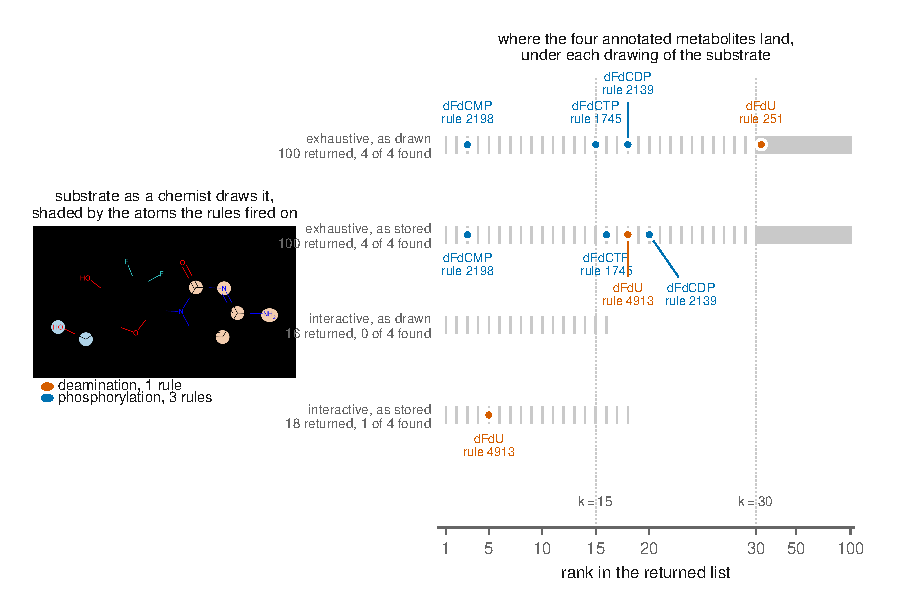
\includegraphics[width=\textwidth]{fig_case}
\caption{The worked example. Left: the substrate as a chemist draws it, with each atom a
firing rule reported shaded in the colour of its transformation. Right: the rank of each of the
four annotated metabolites in each arm's returned list, every returned candidate drawn as a tick,
under both drawings of the substrate.}
\label{fig:case}
\end{figure*}

\begin{table*}[t]
\centering\small
\begin{threeparttable}
\caption{The four annotated metabolites of gemcitabine and the rank each is returned at by the two operating modes, with the bank template that produced it.}
\label{tab:case}
\begin{tabular}{lrrrr}
\toprule
 & \multicolumn{2}{c}{interactive} & \multicolumn{2}{c}{exhaustive} \\
\cmidrule(lr){2-3}\cmidrule(lr){4-5}
annotated metabolite & rank & rule & rank & rule \\
\midrule
dFdU, deamination & 5 & 4913 & 18 & 4913 \\
dFdCMP, 5$^\prime$-monophosphate & --- & not produced & 3 & 2198 \\
dFdCDP, 5$^\prime$-diphosphate & --- & not produced & 20 & 2139 \\
dFdCTP, 5$^\prime$-triphosphate & --- & not produced & 16 & 1745 \\
\bottomrule
\end{tabular}
\begin{tablenotes}[flushleft]\footnotesize
\item Rule is the index into the deployed bank. The substrate is drawn as the corpus stores it; the same run on the drawing a chemist would submit returns different ranks, and both drawings are given in Section~\ref{SI-sec:si-case}.
\end{tablenotes}
\end{threeparttable}
\end{table*}


Gemcitabine is annotated in the corpus with four metabolites: the deamination to dFdU that
inactivates it, and the three sequential 5$^\prime$ phosphorylations that activate it.
Figure~\ref{fig:case} and Table~\ref{tab:case} are what the deployed configuration returns for
it, with the transformation behind every hit.

The interactive mode's budget never selects the rules that make the three phosphorylations, so no ranking could have recovered them; the exhaustive mode applies the whole bank and produces all \numCaseExhFound{}, reaching every one of them by rank \numCaseExhDeepest{}. That last figure is
past the budget this paper reports: \numCaseExhPastfifteenWord{} of the
\numCaseExhFoundWord{} are recovered only beyond $k=15$, so at the reported budget this molecule is one hit and not four. The
class it illustrates is the one the bank is weakest on. At the reported budget the exhaustive arm recovers none of the comparison set's \numChemDeamRefs{} annotated deaminations and the best comparator recovers most of them (Table~\ref{tab:si-chemistry}).  The division the sweep shows across
\numPopulationN{} substrates is visible on this one molecule: the interactive mode is right about what
it emits and runs out, and the exhaustive mode keeps having candidates.

The attribution is what a score cannot supply. All three phosphorylations fire at the same
substrate atoms, the 5$^\prime$ hydroxymethyl, under three different rules, and the deamination
fires on the pyrimidine ring, so the output states which transformation is claimed and where,
and a candidate can be rejected on mechanistic grounds. On the stored drawing all four rules are mined, so the part of the bank with no expert provenance is what carries this molecule; on the drawing a chemist would use, a curated template finds the deamination instead, and later in the list (Section~\ref{SI-sec:si-presentation}). Which templates carry a molecule is itself a function of how the molecule is drawn,
and Figure~\ref{fig:case} shows both.

\subsection{Which design choices were selected on which population}

Every deployed choice is a registered hypothesis with a threshold and a falsification condition,
tested where it was not selected (Table~\ref{tab:hyp}). Ten of the sixteen registered are checked
here. Six are confirmed and three failed, each on the falsification condition it was written
with; the tenth was measured rather than adjudicated, because its threshold was fixed in advance
and its population was not. The remaining six are registered against work this paper does not report and are stated
with their thresholds, so that a later result on any of them cannot rest on a threshold chosen
afterwards. Section~\ref{sec:limitations} states which of the seven confirmations a stricter
reading leaves undecided.

\begin{table*}[t]
\centering\footnotesize
\begin{threeparttable}
\caption{Every deployed choice as a prediction fixed before it was checked: what was fixed, the threshold, the value measured, the population it was checked on, and what the check returned.}
\label{tab:hyp}
\begin{tabular}{@{}lllllp{0.125\textwidth}l@{}}
\toprule
 & what was fixed & threshold & measured & tested on & verdict & register \\
\midrule
P1 & rank fusion instead of a score product & $+0.05$ & $+0.0733$ & validation & confirmed; threshold inside interval & H7 \\
P2 & candidate pool capped at 100 & $+0.015$ & $+0.0260$ & validation & confirmed; threshold inside interval & H9 \\
P3 & rule budget of 30 & $\le +0.05$ & $+0.0092$ & validation & confirmed on validation; not on the comparison set & H10 \\
P4 & emit the whole pool, no threshold & 0 cells & $0$ & grid $5\times11$ & confirmed & H11 \\
P5 & group score as a third ranking & $+0.02$ & $+0.0256$ & comparison set$^{\dagger}$ & measured, not adjudicated in advance; threshold inside interval & H12 \\
P6 & group score, groups emitted as blocks & $+0.05$ & $-0.1188$ & comparison set$^{\dagger}$ & failed & H8 \\
P7 & group score as a gate before fusion & $+0.02$ & $-0.0195$ & comparison set$^{\dagger}$ & failed & H14 \\
P8 & standardise survivors only & $\ge 10\times$ & $2.95$ & validation & failed & H13 \\
P9 & survivors, tautomer budget 200 & $<10$ s & $5.28$ & validation & confirmed & H15 \\
P10 & composite share, both instruments & $\ge 0.134$ & $0.2212$ & mined bank & confirmed & H16 \\
\bottomrule
\end{tabular}
\begin{tablenotes}[flushleft]\footnotesize
\item P8's figure is a speed-up factor, P9's a median in seconds and P10's a share of the mined bank; the rest are differences in micro recall at a budget of 15. $^{\dagger}$ marks the three whose threshold was fixed in advance but whose population was not. The last column carries each row's identifier in the released register, which numbers the predictions in the order they were written rather than the order they are read.
\end{tablenotes}
\end{threeparttable}
\end{table*}


\subsection{Runtime}

\begin{figure*}[t]
\centering
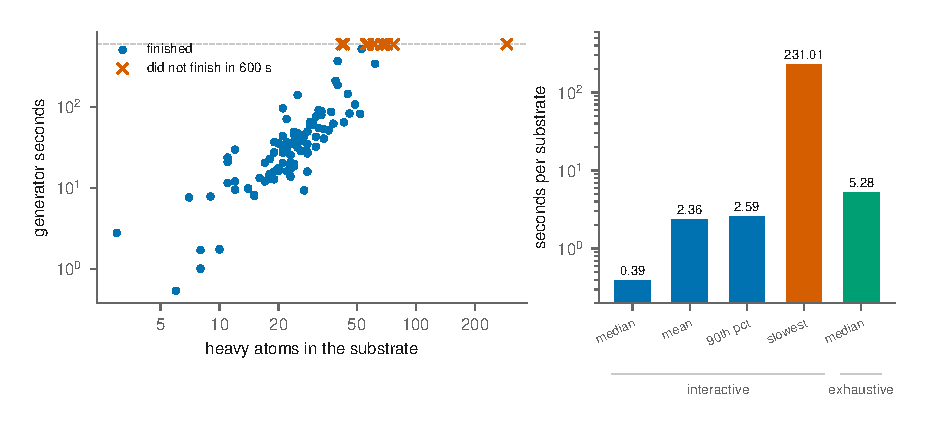
\includegraphics[width=\textwidth]{fig_cost}
\caption{Left: generator seconds against substrate size at the whole bank, both axes logarithmic,
with the substrates that did not finish inside the \numCostDeadline{}-second deadline drawn on the
dashed line marking it. Right: wall-clock seconds per substrate for each operating mode on the
validation split, log scale; the first four bars are the interactive mode's median, mean, ninetieth
percentile and slowest substrate, the fifth the exhaustive mode's median.}
\label{fig:cost}
\end{figure*}

The binding constraint is product standardisation, run once per product of every template; three other candidates were tested and rejected by measurement (Section~\ref{SI-sec:si-runtime}).

Two registered predictions followed. Standardising only the survivors (P8) freed recall but missed its registered speed-up threshold (Table~\ref{tab:hyp}). Adding a
tautomer enumeration budget of \numHOneFiveBudget{} (P9) passes both halves, taking the median from
\numHOneThreeTimeBefore~s to \numHOneFiveTime~s against a registered target below ten, at a recall
loss of $\numHOneFiveRecallDiff$ against a cap of $0.01$.

Cost is reported at the tail as well as at the median, because a service is used at both. The interactive mode's tail is far heavier than its median (Table~\ref{tab:modes}), so a service answering a web form should impose a deadline and fall back rather than size itself on the median.

\subsection{The ceiling, and how much of it is the corpus}
\label{sec:ceiling}

Applying the whole bank to every test substrate recovers \numCeilingCoverage{} of references in
one step, under the same tautomer-aware matching criterion the comparison defaults to and on the
same evaluated test set, leaving \numCeilingUncovered{} uncovered. That count is measured with hydrogens implicit through the firing loop a caller runs; a loop and a hydrogen convention together are the \emph{instrument}, and the bound moves with it. The remainder divides by the reaction-centre change it requires: \numCeilingNovel{} need
a transformation type the bank does not hold, \numCeilingKnown{} need a type it holds whose rule
did not fire, and \numCeilingUntypeable{} cannot be typed. Those \numCeilingNovel{} are
\numBoundShortfallsharemax{} of the \numCeilingUncovered{}, the upper end of the bound this paper
states on how much of the shortfall is chemistry the corpus never contains; the lower end,
\numBoundShortfallsharemin{}, is derived from the marginals and both counts are in
Section~\ref{SI-sec:si-typeoverlap}.

The coverage figure is what orients the two directions this work could go next, so it is worth
putting beside the recall. On the comparison set the ceiling is \numHeadroomCeiling{} and the exhaustive
arm at a budget of fifty reaches \numHeadroomReached{}, which is \numHeadroomSharePct{} of what
the bank can reach. The headroom a better ranking could take is \numHeadroomRanking{}; the
headroom no ranking can take, because the bank does not produce those structures at all, is
\numHeadroomCoverage{}. The census below is about the second and the larger.

What the ceiling counts is one application of one template and not one enzymatic step, which
matters for how the number reads. The
annotation itself is not all single steps: applying the composite instruments to the references
rather than to the templates, \numRefstepEither{} of the \numRefstepTyped{} pairs those
instruments can type, \numRefstepEithersharePct{}, are flagged as reached in more than one
turnover and recorded by the corpus as one pair.  A hit on one of those is a single template standing in for
several turnovers, so \numCeilingCoverage{} is not the share of annotated metabolism one enzymatic
step reaches.

How hydrogen is presented to a template changes what fires, so the convention is named here
rather than left to the code. The bound stated above, \numCeilingUncovered{} uncovered, is
measured with hydrogens implicit through the loop a caller runs, which is the convention every
deployed firing path uses. The three other counts are these. A bound that moves with the
instrument has to be read with that movement beside it.
Measured instead through the loop that audits both conventions from one code path, implicit
hydrogens leave \numCeilagreeAuditimplicitUncovered{} uncovered and hydrogens made explicit with
the templates completed to match leave \numCeilagreeAuditcompletedUncovered. Choosing the
convention per template, which no caller can request, leaves \numCeilagreeDispatchUncovered. A
fourth arm, hydrogens made explicit without completing the templates, is an incomplete loop rather
than a convention and leaves \numHydUncoveredexpanded{} uncovered, more than any of the other
three; the instrument's own record excludes it.

The first two are the same convention measured through two different loops, and they disagree by
\numCeilagreeDisagreementWord{} references because the two loops clean products differently. All four span \numCeilagreeSpread{} references of
\numHydReferences{}, which is \numCeilagreeSpreadshare{} of recall and so
\numCeilagreeSpreadofmarginPct{} of \numCeilagreeNarrowestmargin{}, the narrowest
margin that separates from zero anywhere in the comparison table, so the choice of instrument
cannot decide a claim here. The residual dependence of the bound on the convention, measured per template, is
$\numHydResidual{}$, 95\% CI $[\numHydResiduallo{}, \numHydResidualhi{}]$, an interval excluding
zero: the bound is convention-dependent, by \numHydResidualrefs{} references in
\numHydReferences{}.

The \numCeilingNovel{} misses of absent type collapse into \numCensusTypes{} distinct types, of
which \numCensusOnce{} occur once and carry \numCensusOnceSharePct{} of the mass. The objection that
this is a consequence of how finely a type is defined is answered by varying the definition. What
that answer covers should be said exactly: it covers the \numCeilingNovel{} misses of absent
type and not the other \numCeilingKnown{} plus \numCeilingUntypeable{} of the
\numCeilingUncovered{}. A miss whose type the bank holds and whose rule did not fire is an implementation failure by
construction. Three of the \numCeilingKnown{} were recovered by relaxing convention-dependent
primitives, so that arm is not invariant to anything.

\begin{table*}[t]
\centering\small
\begin{threeparttable}
\caption{The novel-type gap against the definition of a type.}
\label{tab:grain}
\begin{tabular}{lrrrl}
\toprule
definition of a type & types & once & mass & names a \\
 & & & & transf. \\
\midrule
multiset of changed bonds, with counts & 312 & 294 & 87.2\% & yes \\
the same, counts dropped & 284 & 247 & 73.3\% & yes \\
element pairs that take part & 69 & 30 & 8.9\% & \textbf{no} \\
number of bonds that change & 44 & 9 & 2.7\% & \textbf{no} \\
\bottomrule
\end{tabular}
\begin{tablenotes}[flushleft]\footnotesize
\item Each row is one definition, coarsening downward. \emph{types} is how many distinct types the misses of absent type collapse into under it, \emph{once} how many of those are seen exactly once, and \emph{mass} the share of the gap those once-only types carry. The last column says whether a type under that definition still determines a product. The tail is present wherever it does and collapses only below that.
\end{tablenotes}
\end{threeparttable}
\end{table*}


\begin{figure*}[t]
\centering
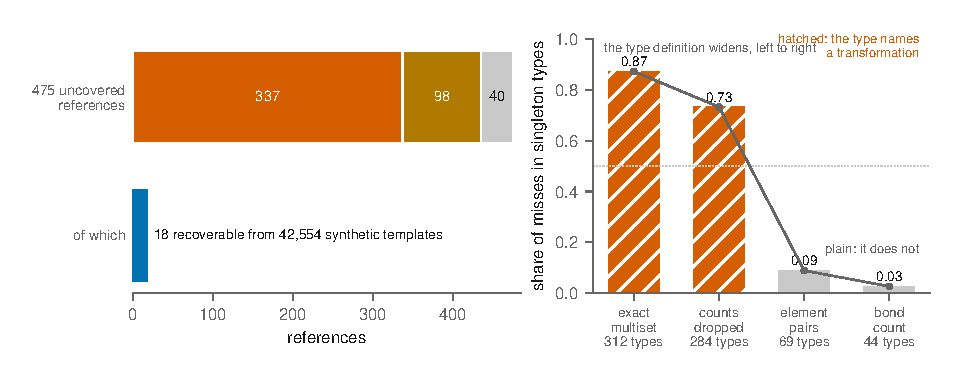
\includegraphics[width=\textwidth]{fig_ceiling}
\caption{Left: where the \numCeilingUncovered{} uncovered references go, and how many of them a
library of \numUsptoTemplates{} synthetic templates could supply. Right: the share of the
novel-type gap sitting in types seen exactly once, against four definitions of a type; the label
above each bar is that share and the count under each tick is how many distinct types the
definition yields. The hatched bars are the definitions under which a type still names a transformation, so the
distinction does not rest on colour.}
\label{fig:ceiling}
\end{figure*}

The tail holds at every granularity at which a type still determines a product and collapses only
where it stops doing so (Table~\ref{tab:grain}, Figure~\ref{fig:ceiling}). What the table does
not make definition-free is the share itself: \numCensusOnceSharePct{} is read under our own
definition of a type, and a coarser one collapses it. What it supports is the different claim
that the bound is invariant to the definition across the whole range in which that definition is
meaningful. That makes the census of the gap a fact about the annotation corpus rather than about
our own choice of definition; what the engine contributes is the hydrogen convention measured
above.

Nor is the missing chemistry available in the largest reaction library we hold. Typing
\numUsptoTemplates{} retrosynthetic templates \citep{Maziarz_2025, Tanovic_2026} in the
metabolic direction gives \numUsptoTypes{}
types, of which \numUsptoHit{} are among the \numCensusTypes{} missing, carrying \numUsptoMass{}
of the \numCeilingNovel{} misses. It is a thin intersection, \numUsptoSanity{} of the bank's \numBankTypes{} types, so the \numUsptoHit{} is a looser statement than it looks.

\section{Discussion}
\label{sec:discussion}

\subsection{Where the advantage is, and where it is not}

The comparison does not produce a winner. SyGMa recovers more at the head of the list, and at
$k \le 5$ the interval separates against GRAIL. GRAIL continues to improve at budgets where the
other systems stop. At a budget of three candidates SyGMa is the better choice; at fifty this
work's exhaustive arm recovers more, and against SyGMa it does so for a reason that survives
matching the two on list length, while against MetaTox and MetaPredictor it does not.

The first half of that is a result about the field and not about this system. SyGMa is the
oldest and by far the smallest method in the comparison, \numSygmaRules{} published rules against
this bank's \numBankRules{}, and at every budget of five or fewer it recovers more of the
annotated metabolites than any other method here, including two published since. A chemist
reading a short list is working at exactly those budgets. That is visible only because the budget is swept.
At a budget of fifty the ordering reverses, the exhaustive arm ahead of every comparator (Table~\ref{tab:sweep}).

The division has a consequence for how such tools are compared. A single recall figure at a
single budget would have named a different winner depending on which budget its author chose,
and each of those choices would have been defensible. That is the case for reporting the sweep
rather than a single cell, and it is made here on this system's own numbers.

\subsection{Choosing an operating point}
\label{sec:offers}

The two modes are two settings of one rule budget, and which to run is decided by the budget the
service answers at rather than by a default. Below about ten candidates the interactive mode is the
right setting and the faster of the two by the margin Figure~\ref{fig:cost} reports;

Beyond a short list that setting is the weaker one, and the cause is the pool rather than the
ranking. It returns far fewer candidates than MetaTox, and by $k=20$ many of its lists have already ended; a list that has ended cannot gain a hit from a wider window, so it trails MetaTox at every budget above fifteen with the interval excluding zero (Tables~\ref{SI-tab:si-short} and~\ref{SI-tab:si-intervals}). A service deployed in that mode would recover
less than the system it replaces wherever it answers with thirty candidates or more.

A service answering with thirty or fifty candidates must therefore either run the exhaustive mode,
which leads MetaTox at both, or raise the rule budget, which is the same knob the exhaustive mode
turns to its limit. On validation that gain appears at an output budget of thirty and not at fifteen (Section~\ref{SI-sec:si-budget}). Either way it pays
in runtime and in what a caller receives: at fifty the exhaustive arm's precision is
\numPrecBankFiveZero{}, about thirty wrong structures for each right one. A list of that length is why the next property matters more than the recall figure does.

\subsection{What is and is not distinctive}

What distinguishes this system is not that it reports a site but that the site is audited.
BioTransformer's output names the reaction and the enzyme behind each structure it returns, and
MetaTox's method reports a biotransformation type and a site of metabolism \citep{Rudik_2017}, so
reporting one is the norm rather than a contribution. Checking it against the atoms that actually
changed, against a null of the same size, is not done anywhere in this literature that we can find,
and Section~\ref{sec:site} is that check. Nor is ordering the whole output, which \numArmreturnOrderingWord{} of the \numComparatorsNWord{} comparators also do. What is left, and it is the property this
paper rests on, is that every evaluation choice is declared with every cell of the resulting grid
reported.

\subsection{What the numbers do not support}

GRAIL does not lead at the tight budgets.  The established lead is the exhaustive arm's, at $k=30$ and $50$. The system is not compared against the 2025--26 wave, because that wave cannot be run as
released: of \numComparatorsUnavailableWord{} such systems none ships a runnable metabolite
predictor \citep{Larsson_2025, Zhou_2025, Zhou_2026, Chavan_2026}, one of them releasing weights
whose reaction module was withdrawn, and the Supporting Information says what each is missing. No ranking in this literature can presently be verified independently, which
is the concrete case for leaderboards releasing per-item predictions rather than aggregate scores
\citep{Rodriguez_2021, Mishra_2021}. Precision figures are bounded by annotation completeness. And the advantage at
wide budgets is partly a statement about output length on all sides rather than about ranking.

The argument made here about other people's figures was turned on this work's own release, and it
found settings that decide a number and were not declared. Six of them: the aggregation of the templates reaching one candidate, the fusion constant, a rule gate the released checkpoint carries, a set of pools scored by a checkpoint this repository no longer ships, the drawing of the substrate, and the pool cap. Each is declared and measured here rather than described, which may be read either way: as the
discipline doing its work, or as a measure of how easily an undeclared setting survives even in a
paper whose subject is undeclared settings. The second reading is why the first is worth
reporting.

\subsection{The ceiling bounds this formulation, not the task}

The shortfall is a property of the corpus the templates are mined from, and it is measured directly
rather than argued from the bank's coverage: of the \numCeilingUncovered{} references one
application of this bank fails to reach, between \numBoundShortfallsharemin{} and
\numBoundShortfallsharemax{} are of a type the training annotation never holds. That is a bound rather than a point, and Section~\ref{SI-sec:si-typeoverlap} gives the counts it rests on.

Extending coverage therefore requires new reaction corpora, and the census narrows the search.
Synthetic corpora are excluded by measurement, which leaves enzymatic and regulatory sources. The
regulatory ones are the interesting half: metabolite identifications from radiolabelled human
ADME studies are human \emph{in vivo} data on exactly the population predicted here, they have
been used to benchmark this class of tool \citep{Gao_2026}, and they are, to our knowledge, not
systematically mined as a source of rules. Whether the same bound binds a predictor that applies no templates at all is not measured here.

What the bound licenses is worth saying plainly, because the corpus it is a property of has two
defects this paper also reports. Its assembly cannot be reconstructed, and the one source held on
disk shows the selection was not blind to chemistry. So the bound says: extending the bank by
mining \emph{this} corpus harder cannot close the shortfall, because the chemistry is not in it. It
does not say what fraction of human metabolism is of a type no corpus contains, and it cannot,
because that would need a corpus whose assembly is recoverable and whose selection is documented.
What makes the narrower statement worth having anyway is that this corpus is assembled from the
four sources this field trains on, so a bank mined from any of them inherits the same absence
unless the assembly is changed. The claim is about a training corpus and about the practice of
mining it, not about metabolism.

\section{Limitations}
\label{sec:limitations}

Applying one template once is not the same as one enzymatic step. The registered instrument counts
core-incident edits and calls a template composite at \numCompositeThreshold{} or more, above every
single enzymatic turnover; it flags \numCompositeEditsharePct{} of the mined templates it can
score, clearing the bar registered prediction P10 set at \numCompositeBarPct{}. A second instrument
counting reaction-centre loci flags \numCompositeLocisharePct{}, but errs in both directions with
neither error measured, so its share is neither a floor nor a bound; the two agree on only
\numCompositeBoth{} templates (Section~\ref{SI-sec:si-singlestep}). The coverage ceiling here is
therefore a one-template ceiling and not a one-enzyme one, and the composite share is why a second
application of the bank buys little: a fifth of the mined bank already carries the compositions a
second pass would have to discover. A depth-two probe put the lift in the low percent at several
times the candidate cost, and no figure from it is quoted, because its result file names no
producer and predates the provenance apparatus the rest of this work is held to.

Both learned stages are trained short of what the split allows, on a subsample of it and with early stopping that never engaged, which is an underfitting signature and not a converged run; retraining on the full split is not reported (Section~\ref{SI-sec:si-retrain}).

The register is weaker than its count of confirmations suggests. Three of the six confirmed
predictions clear the falsification condition as written, which compares a point estimate to a
threshold, and not the stricter reading that asks the whole interval to clear it. P1 and P2 have
their threshold inside their own interval, and so does P5. What the data establish for those three
is that the effect exceeds zero, not that it exceeds the registered bar. P5 is weaker again, and
the register is what shows it: its threshold was fixed in advance but its population was not, and
it was adjudicated on the comparison set, which is derived from the test split and was recorded
afterwards. Table~\ref{tab:hyp} calls that a measurement rather than a confirmation, which is why
it is not one of the six. P3's threshold
is in any case a property of the budget requested rather than of the system.

Two reported quantities are bounded by things outside the system. Precision is bounded by how
completely the corpus annotates, so every precision figure here is a lower bound of unknown depth;
and every method runs out of candidates at wide budgets, so the widest columns measure list length
on all sides as much as ordering. The comparison population is the \numPopulationN{} substrates every method has an entry for, a quarter of the evaluated test split, and how that quarter was drawn is not recorded (Section~\ref{SI-sec:si-population}). Two comparators, BioTransformer and GLORYx, are built on sources this corpus is assembled
from, which favours both and is not corrected for.

The deployed configuration is not the best one this work knows of. A blend that discounts
duplication beats the released noisy-or on the validation draw at every budget from one to
\numAggvalHybridwinsmax{}, with the interval excluding zero, which includes the budget the headline
is read at (Section~\ref{SI-sec:si-aggregation}). The release keeps the noisy-or because every
number here is measured under it and switching would leave the paper describing a system nobody
ran; the choice is a parameter rather than a retraining, so the blend can be selected without
retraining anything. GLORYx is the one arm not run on this machine: the models it needs are not distributed with its
source, so its column comes from the service its authors operate
(Section~\ref{SI-sec:si-comparators}). Stereochemistry and protonation are bounded rather than priced. \numStereoSharePct{} of annotated
pairs produce a metabolite carrying a stereogenic element its substrate does not have, and
\numChargeSharePct{} of annotated metabolites carry a formal charge. The criterion sweep cannot
price a configuration-aware criterion, because no reference in this corpus carries a configuration
for one to read. What separates the two settings that differ in that layer, on this annotation, is
protonation and not stereochemistry (Section~\ref{SI-sec:si-sensitivity}).

No measurement of a system here is external. Every figure is measured on one corpus assembled from
four sources, of which the only published reference set is one of the four, so a held-out split of
it is not an independent test of the chemistry. The set that would serve is metabolite
identifications from radiolabelled human ADME studies, already used to benchmark this class of tool
\citep{Gao_2026}; measuring a system here on one is not possible from what that benchmark
publishes, because its reference structures appear only as drawings. Until it is, the comparison
establishes an ordering within a corpus and not a ranking of the methods.

The claim about evaluation is a different matter, and it is checked outside this corpus.
\citet{Gao_2026} deposited the prediction files the \numExtbudgetArmsWord{} predictors they
benchmarked returned, so what each emitted is counted rather than inferred. Counted, across their
\numExtbudgetDrugs{} drugs the axis that benchmark leaves undeclared spans a factor of
\numExtbudgetRatio{}, from \numExtbudgetNarrowest{} candidates per drug to
\numExtbudgetWidest{}: an undeclared quantity varying twelvefold between the arms of a
comparison is part of what the comparison measures. The arms that emit more score higher. Shuffling emission among the arms of a drug, which breaks only which arm is paired with which emission, does not reproduce that association (Section~\ref{SI-sec:si-external}).

It lives mostly between the arms, which is the level at which a benchmark orders them. It is not the whole story and
this paper's argument does not need it to be: ordering the arms by what they emit does not
reproduce ordering them by recall, one arm returning fewer candidates than another and recovering
more. So output size is a confound in that benchmark rather than its content, which is the same
thing this paper says about its own budget axis, and the remedy is the same, to declare the axis
and vary it.

\section{Conclusions}
\label{sec:conclusions}

GRAIL predicts metabolite structures by selecting templates from a bank of \numBankRules{} reaction
rules, applying them, and ranking the products by a reciprocal rank fusion of two learned scores.
How those two scores are combined mattered more than what produced them: replacing their product
with the rank fusion gained more recall than any architectural change tested here. Every prediction
carries the template that produced it and the atoms it acted on, so a candidate can be judged on
mechanistic grounds. Measured against the published predictors that could be run on the same
substrates, the comparison divides by output budget rather than resolving into an ordering, and
that division is the result: a single recall figure would have named a different leader depending
on decisions its author never had to state. Reporting the whole grid is what makes the comparison
checkable, and releasing every arm's per-substrate predictions is what lets a third party
recompute it.

What one application of one template bank cannot reach is mostly chemistry the corpus does not
contain: between \numBoundShortfallsharemin{} and \numBoundShortfallsharemax{} of the
\numCeilingUncovered{}-reference shortfall is of a type the training annotation never holds.
Enlarging this bank from this corpus would not supply that chemistry. The bound is therefore a
property of the corpus this field trains on and not of any one bank.

\begin{suppinfo}

The Supporting Information is available free of charge on the ACS Publications website.

Corpus, splits and leakage audit; what kind of molecules these are; the five matching criteria and the comparison's sensitivity to
the choice among them; the parent-drop convention per arm; every candidate count the paper prints;
precision at every budget; every comparison difference with its paired interval, at matched list
length and under the other aggregation; how the substrate is drawn and where that changes a
verdict; the rule bank, its mining and the provenance of each collection; what the rule budget
buys and two parameters of the ranking, swept; architecture, training and settings of both learned
stages; whether the site a prediction names is the site that changed; what each method recovers by
transformation class; whether the missing chemistry is the corpus's or the bank's, and whether
template discovery has saturated; how much of the annotation is one enzymatic step; the sixteen
registered predictions; group ranking and its oracle; the stage ablations; the choice of evaluation
population; the worked example on both drawings; runtime methodology; comparator versions and
digests; the evaluation claim checked against an independent benchmark; provenance and reproduction
procedure (PDF)

\end{suppinfo}

\section{Data and Software Availability}

Source code, the deployed checkpoints, the released rule bank, the split manifest, the annotated
references every recall figure is measured against, the frozen per-substrate predictions of every
comparator, the evaluation harness, the provenance sweep and the preregistration with every
hypothesis and its outcome are at \texttt{github.com/doctawho42/GRAIL}, and are available to
reviewers at submission. The train and validation candidate pools are deposited at \ZenodoDoi{}.

The released bank is not the measured bank. This paper's figures are measured on
\numRelbankMeasured{} templates, of which \numRelbankRemoved{} are also in BioTransformer's
published set; that distribution's licence grants redistribution with attribution and reserves
permission for \emph{commercial} use, so the shipped bank drops them as a courtesy rather than an
obligation and \numRelbankReleased{} ship. The removal is free: every reference those templates
reach is reached by another in the bank. Dropping them from the bank is not the same as not
carrying them, and of \numRelbankCarrierscanned{} tracked files \numRelbankCarriersWord{} hold at
least one, which a check reports rather than the repository asserting otherwise. The repository's
licence is \RepoLicence{}, which is what the remaining GPL templates permit rather than a
preference, and \texttt{NOTICE.md} carries the decisions file by file.

The corpus, whose four sources and versions Section~\ref{sec:populations} names, is not
redistributed as a corpus: ShareAlike and NonCommercial terms cannot
both be satisfied by one derivative, so its licence is \CorpusLicence{}. What is released instead
is the evaluated test substrates as structures and their annotated metabolites as the descriptors
the matching criteria are decided by, which lets anyone without those licences recompute every
recall figure and every cell of the criterion sweep; a check reports zero disagreements between the
two readings. Releasing the checkpoints is the bar this paper applies to others: a system whose weights cannot
be obtained cannot be compared against, which is why one of the \numComparatorsUnavailable{}
systems of 2025--26 is excluded here.
Section~\ref{SI-sec:si-corpus} states what can and cannot be rebuilt, and the one step that
cannot be reproduced.

\section{Author contributions}

N.L.P. designed the system, wrote the code, ran every experiment reported here and wrote the
manuscript. A.V.R. reviewed the manuscript and will deploy the released model as a service on
\texttt{way2drug.ru}.

\begin{acknowledgement}

\Funding{}

\AIUse{}

\end{acknowledgement}

\section*{Notes}

A.V.R. is an author of MetaTox \citep{Rudik_2017}, the incumbent system this work is
compared against and sets out to replace, and will deploy the released model as a service on
\texttt{way2drug.ru}, which also hosts MetaTox. The authors declare no other competing interest,
financial or otherwise. Any interest that relationship could create runs against this work rather
than for it, and what the MetaTox arm consists of, together with what the service does not expose
to a submitter, is stated in the Supporting Information.
